
\documentclass{article}

\usepackage[left=1.8cm,right=1.8cm, top=2cm, bottom = 2cm]{geometry}
\usepackage{amsfonts}

\usepackage{amsmath}
\usepackage{xcolor}

\usepackage{tikz}
\usepackage{subfigure}

\usepackage{pgfplots}

\pgfplotsset{compat=1.10}
\usepgfplotslibrary{fillbetween}
\usetikzlibrary{patterns}



\pagestyle{empty}

\setlength{\tabcolsep}{15pt}


\newcommand{\deriv}[3][]{\frac{\mathrm{d}^{#1}#2}{\mathrm{d}#3^{#1}}}
\newcommand{\diff}{\;\mathrm{d}}

\newcommand{\norm}[1]{\left|\kern-1pt\left|#1\right|\kern-1pt\right|}
\newcommand{\bra}[1]{\left\langle #1 \,\right|}
\newcommand{\ket}[1]{\left|\, #1\right\rangle}
\newcommand{\braket}[2]{\left\langle #1 \mid #2 \right\rangle}




\begin{document}

\title{The Routh-Hurwitz Test}
\date{}

\maketitle
\thispagestyle{empty}

\Large

\vskip -10mm

\textbf{\underline{Objective: To practise using the Routh-Hurwitz Criterion.}}



\vspace{5mm}





Suppose a system with unity gain negative feedback has open-loop transfer function
\[\frac{k}{s(s+1)(s+2)},\]
where $k$ is some real constant. Find the range of values of $k$ for which this system is stable.


\clearpage


Show that the systems below are equivalent. Use the Routh-Hurwitz text to determine whether or not the system is stable.

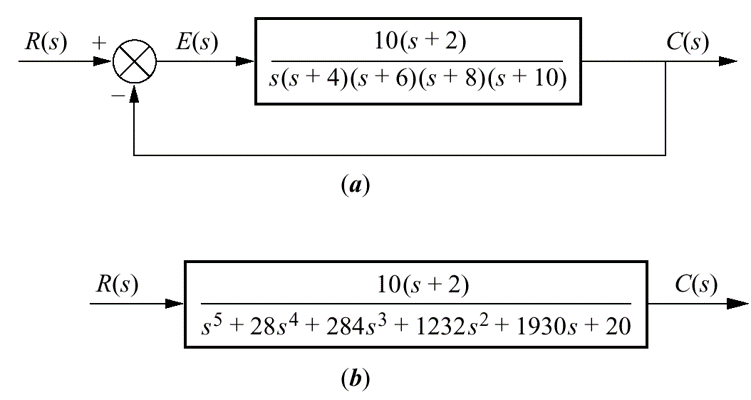
\includegraphics[scale=0.7]{HardPoles.png} 














\end{document}